\documentclass[a4paper]{article}
\usepackage[a4paper,margin=0mm]{geometry}
\usepackage{fontspec}
\usepackage{unicode-math}
\usepackage{tikz}
\usetikzlibrary{fit,calc,positioning,arrows.meta}
\usepackage[table]{xcolor}
\usepackage[absolute]{textpos}
\usepackage{array}

\setmainfont{Libertinus Serif}
\setsansfont{Libertinus Sans}
\setmathfont{Libertinus Math}

\definecolor{accent}{HTML}{602785}
\definecolor{badge}{HTML}{B8A0C8}
\definecolor{ink}{HTML}{2A2E30}

\setlength{\TPHorizModule}{1mm}
\setlength{\TPVertModule}{1mm}
\setlength{\parindent}{0pt}
\pagestyle{empty}

\newcommand{\topicheader}[2]{%
\begin{textblock*}{194mm}(16mm,10mm)
\begin{tikzpicture}
\node[fill=accent,text=white,font=\sffamily\bfseries\fontsize{13}{13}\selectfont,
      minimum width=9mm,minimum height=9mm,inner sep=0pt] at (4.5mm,-4.5mm) {#1};
\node[font=\sffamily\bfseries\fontsize{15}{16}\selectfont,text=ink,anchor=west] at (12mm,-4.5mm) {#2};
\end{tikzpicture}
\end{textblock*}
\begin{textblock*}{194mm}(16mm,22.5mm)

\begin{tikzpicture}
\fill[accent] (0,0) rectangle (194mm,0.5mm);
\end{tikzpicture}
\end{textblock*}
}

\newcommand{\pagekicker}[1]{%
\begin{textblock*}{100mm}(16mm,25.5mm)
\begin{tikzpicture}
\node[fill=ink,text=white,font=\sffamily\bfseries\fontsize{8}{8}\selectfont,
      inner sep=2.2pt,rounded corners=1pt] {\MakeUppercase{#1}};
\end{tikzpicture}
\end{textblock*}
}

\newcommand{\videobanner}[1]{%
\begin{textblock*}{178mm}(16mm,25.5mm)
\begin{tikzpicture}
\fill[accent] (0,0) rectangle (178mm,-10mm);
\draw[white,line width=0.6pt] (3mm,-1.7mm) rectangle (11.5mm,-8.3mm);
\node[white,font=\sffamily\fontsize{4}{4.4}\selectfont,align=center] at (7.25mm,-5mm) {QR\\CODE};
\node[white,font=\sffamily\bfseries\fontsize{9.5}{11}\selectfont,anchor=west] at (16mm,-5.6mm) {WATCH THE VIDEO BEFORE YOU SOLVE};
\node[white,font=\sffamily\fontsize{7.5}{8}\selectfont,anchor=east] at (174mm,-5.6mm) {YouTube ~\textbullet~ #1};
\end{tikzpicture}
\end{textblock*}
}

\newcommand{\pagefooter}[1]{%
\begin{textblock*}{194mm}(8mm,286.41mm)
  
\begin{tikzpicture}
    \fill[accent] (0,0) rectangle (194mm,0.6mm);
  \end{tikzpicture}
\end{textblock*}
\begin{textblock*}{63.59mm}(8mm,288.27mm)
  {\sffamily\bfseries\color{accent}\fontsize{13}{16}\selectfont SAT 1200+}
\end{textblock*}
\begin{textblock*}{10mm}(188mm,288.27mm)
  \centering{\sffamily\color{accent}\fontsize{14}{16}\selectfont #1}
\end{textblock*}
}

\newcommand{\cardbg}[4]{%
\begin{textblock*}{#3mm}(#1mm,#2mm)
\begin{tikzpicture}
\fill[badge!22,rounded corners=3mm] (0,0) rectangle (#3mm,-#4mm);
\end{tikzpicture}
\end{textblock*}%
}

\newcommand{\pill}[3]{%
\begin{textblock*}{160mm}(#1mm,#2mm)
\begin{tikzpicture}
\node[fill=accent,text=white,anchor=north west,font=\sffamily\bfseries\fontsize{10}{10}\selectfont,
      rounded corners=8pt,inner xsep=5mm,inner ysep=1.8mm] at (0,0) {RULE ~\textperiodcentered~ #3};
\end{tikzpicture}
\end{textblock*}%
}

\arrayrulecolor{accent}
\setlength{\arrayrulewidth}{0.7pt}
\renewcommand{\arraystretch}{1.5}

\begin{document}

% ======================================================================
% PAGE 1
% ======================================================================
\topicheader{11}{Function Composition \& Transformation}
\videobanner{Lesson 11}
\pagefooter{59}
\mbox{}%

% ---- CARD 1: Composition ----
\cardbg{16}{40}{178}{62}
\pill{26}{43}{Composition (kompozitsiya): $f(g(x))$}

\begin{textblock*}{158mm}(26mm,56mm)
{\fontsize{11}{14}\selectfont\color{ink}
Evaluate inside-out: compute $g$ first, then plug the result into $f$.}
\end{textblock*}

\begin{textblock*}{158mm}(26mm,68mm)
{\fontsize{13}{16}\selectfont
$f(x)=3x-2,\ g(x)=x^2+1$: \quad $f(g(2))=f(5)=13$}
\end{textblock*}

\begin{textblock*}{158mm}(26mm,85mm)
{\fontsize{10}{13}\selectfont\color{black!55}\itshape
$f(g(x))\neq g(f(x))$ in general -- order matters.}
\end{textblock*}

% ---- CARD 2: Vertical transformations ----
\cardbg{16}{110}{178}{75}
\pill{26}{113}{Vertical transformations}

\begin{textblock*}{158mm}(26mm,126mm)
{\fontsize{11}{14}\selectfont
\begin{tabular}{|>{\centering\arraybackslash}p{40mm}|p{106mm}|}
\hline
\rowcolor{accent}
{\color{white}\textbf{Form}} & {\color{white}\textbf{Effect}} \\ \hline
$f(x)+k$ & Shifts graph up $k$ (down if $k<0$) -- output changes, not input \\ \hline
$-f(x)$ & Reflects graph over the $x$-axis \\ \hline
\end{tabular}}
\end{textblock*}

\begin{textblock*}{158mm}(26mm,167mm)
{\fontsize{12}{15}\selectfont
$f(x)=x^2-4$: \quad $f(3)+5=5+5=10$, \quad $-f(3)=-5$}
\end{textblock*}

\clearpage

% ======================================================================
% PAGE 2
% ======================================================================
\topicheader{11}{Function Composition \& Transformation}
\pagekicker{Rules sheet -- 2/2}
\pagefooter{60}
\mbox{}%

% ---- CARD 3: Horizontal transformations ----
\cardbg{16}{33}{178}{150}
\pill{26}{36}{Horizontal transformations}

\begin{textblock*}{158mm}(26mm,49mm)
{\fontsize{11}{14}\selectfont
\begin{tabular}{|>{\centering\arraybackslash}p{40mm}|p{106mm}|}
\hline
\rowcolor{accent}
{\color{white}\textbf{Form}} & {\color{white}\textbf{Effect}} \\ \hline
$f(x+h)$ & Shifts graph LEFT $h$ \\ \hline
$f(x-h)$ & Shifts graph RIGHT $h$ -- opposite of the sign \\ \hline
$f(-x)$ & Reflects graph over the $y$-axis \\ \hline
\end{tabular}}
\end{textblock*}

\begin{textblock*}{158mm}(26mm,98mm)
{\fontsize{12}{15}\selectfont
$f(x)=x^2+2x$: \quad $f(x-2)$ at $x=5$ is $f(3)=15$; \quad $f(-x)$ at $x=3$ is $f(-3)=3$}
\end{textblock*}

\begin{textblock*}{100mm}(26mm,115mm)
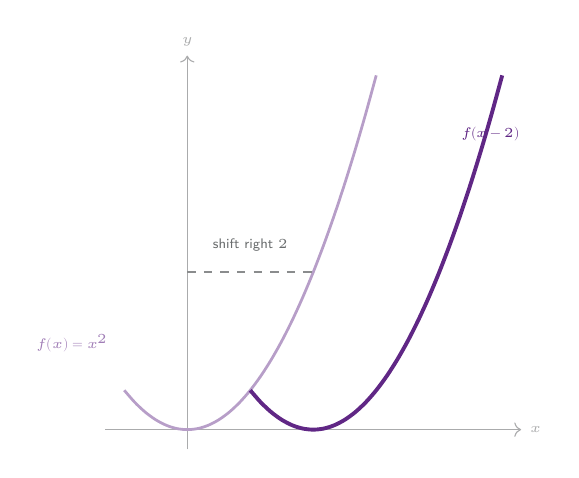
\begin{tikzpicture}[x=8mm,y=5mm]
\draw[ink!40,->] (-1.3,0) -- (5.3,0) node[right,font=\tiny]{$x$};
\draw[ink!40,->] (0,-0.5) -- (0,9.5) node[above,font=\tiny]{$y$};
\draw[accent!45,domain=-1:3,smooth,variable=\x,line width=1pt] plot ({\x},{\x*\x});
\draw[accent,domain=1:5,smooth,variable=\x,line width=1.4pt] plot ({\x},{(\x-2)*(\x-2)});
\node[font=\sffamily\tiny,text=accent!60,anchor=east] at (-1.1,2.2) {$f(x)=x^2$};
\node[font=\sffamily\bfseries\tiny,text=accent,anchor=west] at (4.2,7.5) {$f(x-2)$};
\draw[ink!55,dashed,line width=0.5pt] (0,4) -- (2,4);
\node[font=\sffamily\tiny,text=ink!70] at (1,4.7) {shift right $2$};
\end{tikzpicture}
\end{textblock*}

\begin{textblock*}{158mm}(26mm,170mm)
{\fontsize{10}{13}\selectfont\color{black!55}\itshape
Direction inside the parentheses is always reversed from what it looks like.}
\end{textblock*}

\end{document}
